\documentclass[12pt]{article}

\usepackage{polski}
\usepackage[utf8]{inputenc}
\usepackage{listings}
\usepackage{hyperref}
\usepackage{titlesec}
\usepackage{graphicx}
\graphicspath{{./img/}}
\usepackage{float}
\usepackage{listings}

\titleformat{\subsubsection}
{\bfseries}
{}
{0em}
{}

\begin{document}

\begin{titlepage}
    \centering
    {\scshape\LARGE Politechnika Śląska

    Wydział Automatyki, Elektroniki i Informatyki\par}
    \vspace{1cm}
    {\scshape\Large Computer Programming\par}
    \vspace{1.5cm}
    {\huge\bfseries Binary Tree\par}
    \vspace{2cm}
    \vfill
    author:
    Maciej Krzyżowski\par
    \vfill
\end{titlepage}

\renewcommand*\contentsname{Table of contents}
\tableofcontents
\pagebreak

\section{Introduction}
This project implements a binary tree in the C++ programming language. It is supposed to work on any type of variable or class, provided the ability to compare them. Additionally it should be able to store more than one entry in a single node and keep track of these number of entries. A basic binary tree implementation on integers can be visualised in such a way:

\begin{figure}[H]
    \centering
    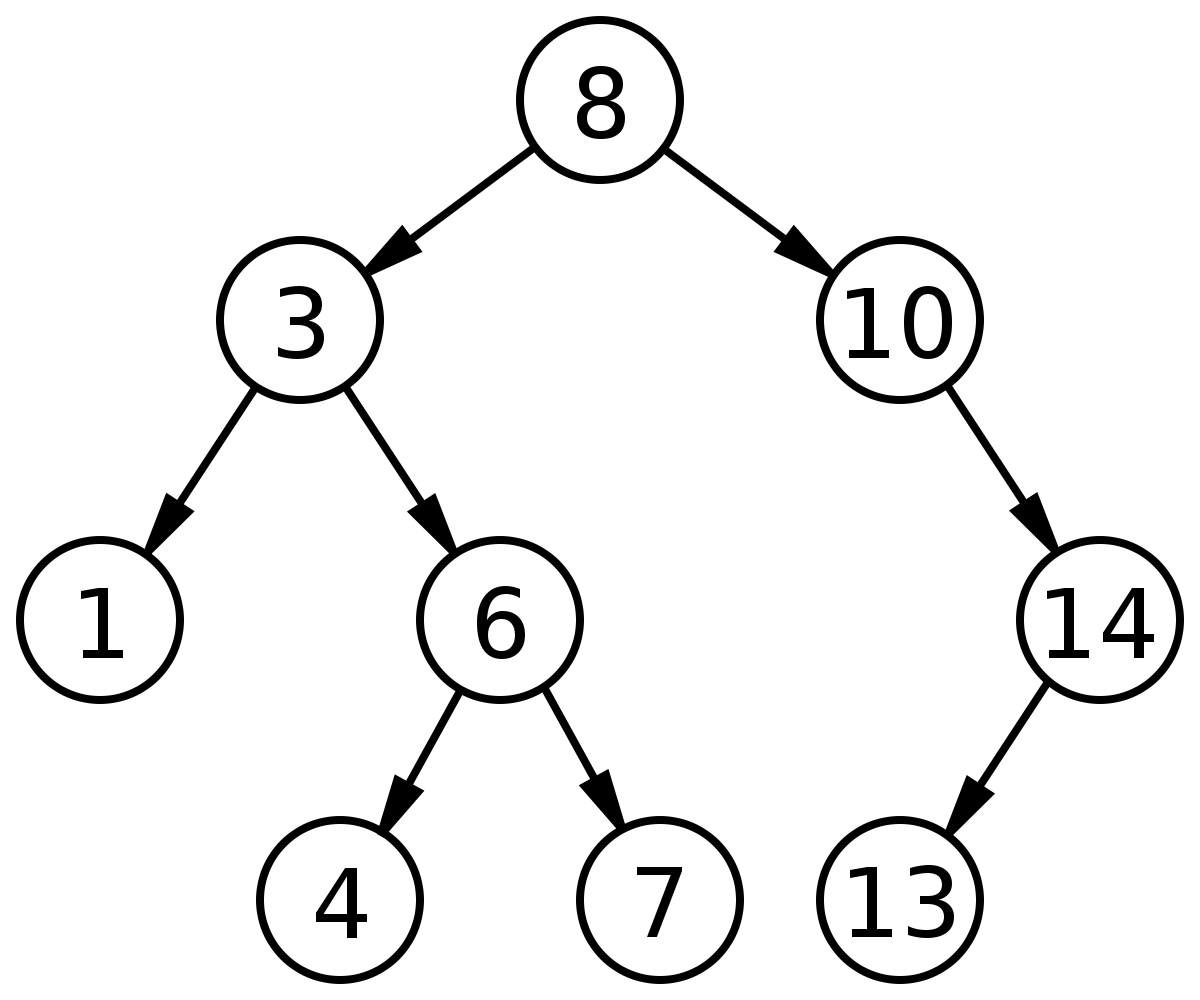
\includegraphics[width=0.75\linewidth]{tree1}
\end{figure}

where every node's value is greater than its left child's value and smaller than its right child's value.

\pagebreak
\section{Requirements}
The implementation is required to meet these requirements:
\begin{itemize}
    \item no use of the STL containers (eg.\ vector, set, list...)
    \item use of the smart pointers
    \item class should contain these methods:
        \begin{itemize}
            \item copy / move constructors
            \item default constructor
            \item assignment / move operators
            \item adding container elements
            \item searching for an element
            \item sorting content
            \item serialization
        \end{itemize}
\end{itemize}

\section{Class Overview}
\subsection{Node Class}
The class \textit{Node} is not very complex. Its members are:
\begin{itemize}
    \item size --- number of entries in one node
    \item val --- a dynamic array storing the value
    \item left and right child
\end{itemize}

It also contains 3 different constructors, a destructor, setting and getting methods and overloaded operators.

\subsubsection{Overloaded Operators}
\begin{footnotesize}
\begin{lstlisting}[language=C++]
template <typename T>
bool Node<T>::operator>(const Node& node) const
{
    return this->val > node->val;
}
template <typename T>
bool Node<T>::operator<(const Node& node) const
{
    return this->val < node->val;
}
template <typename T>
bool Node<T>::operator==(const Node& node) const
{
    return this->val == node->val;
}
template <typename T>
Node<T> Node<T>::operator+(const Node& node)
{
    Node temp;
    temp->val = this->val + node->val;
    return temp;
}
\end{lstlisting}
\end{footnotesize}

Assignment / move operators are presented below, in the section \ref{Creating}.

\subsection{Tree Class}
This class is where the most important operations take place. Apart from methods its only meber is the root of the tree, which is a smart pointer to a object of type \textit{Node}. This class contains every method to meet the requirements.

\pagebreak
\subsubsection{Creating a Tree\label{Creating}}
The class \textit{Tree} has 3 different constructors: one default, and two with an argument: either a template value or an other tree. These constructors look as follows:
\begin{footnotesize}
\begin{lstlisting}[language=C++]
template <typename T>
Tree<T>::Tree(const T _val)
{
    this->root = std::shared_ptr<Node<T>>(new Node<T>(_val));
}

template <typename T>
Tree<T>::Tree(const Tree& tree)
{
    *this = tree;
}

template <typename T>
Tree<T>::Tree()
{
    this->root = nullptr;
}
\end{lstlisting}
\end{footnotesize}

\pagebreak
To make the second constructor work the `=' operator had to be overloaded in such a way for both \textit{Tree} and \textit{Node} class:
\begin{footnotesize}
\begin{lstlisting}[language=C++]
template <typename T>
Tree<T>& Tree<T>::operator=(const Tree& _tree) 
{
    this->root = _tree.root;
    return *this;
}

template <typename T>
Node<T> Node<T>::operator=(const Node& node)
{
    return std::swap(node);
}

template <typename T>
Node<T> Node<T>::operator=(const std::shared_ptr<Node>& node)
{
    this->val = node->val;
    this->left = node->left;
    this->right = node->right;

    return *this;
}
\end{lstlisting}
\end{footnotesize}

\pagebreak
\subsubsection{Inserting}
The most important ability is to insert new elements to the tree. This is done by the method which looks like this:
\begin{footnotesize}
\begin{lstlisting}[language=C++]
template <typename T>
void Tree<T>::insert(const T _val)
{
    if (this->root == nullptr) {
        root = std::shared_ptr<Node<T>>(new Node<T>(_val));
        return;
    }

    std::shared_ptr<Node<T>> temp = nullptr;
    std::shared_ptr<Node<T>> currNode = this->root;
    T currVal;
    while (currNode != nullptr) {
        currVal = currNode->getVal();
        temp = currNode;
        if (_val < currVal) {
            currNode = currNode->left;
        } else if (_val > currVal) {
            currNode = currNode->right;
        } else {
            currNode = currNode;
            break;
        }
    }
    currVal = temp->getVal();
    if (_val < currVal) {
        temp->left = std::make_shared<Node<T>>(_val);
    } else if (_val > currVal) {
        temp->right = std::make_shared<Node<T>>(_val);
    } else {
        temp->incSize();
        temp->setVal(_val, (temp->getSize()) - 1);
    }
    return;
}
\end{lstlisting}
\end{footnotesize}

In this method, the first if-block checks if the tree is empty. In this case it creates a root for a tree and ends its execution. The while-loop in the middle is responsible for finding the proper spot for the new entry, according to therules of a Binary Search Tree (described in the \textit{introduction}). If the place is found, accourding to the same rules, either a new node is created or the entry is placed in the array.

\pagebreak
\subsubsection{Removing}
Removing a node happens within two methods. The first one's only responsibility is to chech if a node with the specified value exists. If it does, it invokes the second method, which does the necessary work. This method's code block looks as follows:
\begin{footnotesize}
\begin{lstlisting}[language=C++]
template <typename T>
std::shared_ptr<Node<T>> Tree<T>::pop_helper(const T _val, 
                                            std::shared_ptr<Node<T>> root) 
{
    if (root == nullptr) { root = this->root; }

    std::shared_ptr<Node<T>> currNode = root;
    if (root == nullptr) { return root; }

    if (root->getVal() > _val) {
        root->left = this->pop_helper(_val, root->left);
        return root;
    } else if (root->getVal() < _val) {
        root->right = this->pop_helper(_val, root->right);
        return root;
    }

    if (currNode != nullptr) {
        if (currNode->left == nullptr && currNode->right == nullptr) {
            currNode = nullptr;
            return nullptr;
        } else if (currNode->left == nullptr) {
            currNode->setSize(currNode->right->getSize());  
            currNode = currNode->right;                    
            return currNode;
        } else if (currNode->right == nullptr) {
            currNode->setSize(currNode->left->getSize());
            currNode = currNode->left;                    
            return currNode;
        } else {                                         
            currNode->setSize(this->min(root->right)->getSize());
            currNode = this->min(root->right);
            root->setVal(currNode->getVal());
            root->right = this->pop_helper(currNode->getVal(), root->right);
            return root;
        }
    }
    return nullptr;
}
\end{lstlisting}
\end{footnotesize}
\pagebreak

The logic behind it is to find the node to be deleted and, accordingly to the number of its children, replace it with one of them. For two children the new node becomes its successor (a minimal node from the right subtree) and for one, it becomes the new node. This method will replace the old root of the tree with a new one.

\subsubsection{Sorting}
Sorting a binary tree results in obtaining a list. This implementation supports both increasing and decreasing sort. Methods responsible for it remove either a minimal or maximal element of the tree, depending if it's a increasing or decreasing sort, insert it to a new tree and finally return the new tree replacing the old one. The available methods are: \textit{sort()} and \textit{rsort()}.

\pagebreak
\subsubsection{Serialization}
Serialization into a file is done by converting the tree into multiple arrays containing values and quantity of entries and boolean values indicating if such node is initialized, to keep the proper order of the nodes. The arrays are obtained using this method:
\begin{footnotesize}
\begin{lstlisting}[language=C++]
template <typename T>
void Tree<T>::valArr(std::shared_ptr<bool[]> isInitialized, 
                    std::shared_ptr<T[]> values, 
                    std::shared_ptr<size_t[]> number, 
                    std::shared_ptr<Node<T>> currNode, 
                    size_t index) const
{
    if (currNode == nullptr)
        currNode = this->root;

    if (currNode != nullptr) {                      
        isInitialized[index - 1] = true;
        values[index - 1] = currNode->getVal();
        number[index - 1] = currNode->getSize();
    } else {
        isInitialized[index - 1] = false;
        return;
    }
    // repeat for the left and right subtree, the index is taken from:
    /*
     *                      1
     *              2               3
     *          4       5       6       7
     *  1 - root
     *  2 and 3 - root's children
     *  etc.
     */
    if (currNode->left != nullptr)
        valArr(isInitialized, values, number, currNode->left, index * 2);

    if (currNode->right != nullptr)
        valArr(isInitialized, values, number, currNode->right, index * 2 + 1);
}
\end{lstlisting}
\end{footnotesize}

\pagebreak
These arrays are then used in the method responsible for outputting to a text file. This method is rather not complicated and is presented below:

\begin{footnotesize}
\begin{lstlisting}[language=C++]
template <typename T>
void Tree<T>::toFile(std::string fileName) const
{
    fileName = (fileName == "") ? "./data/output.txt" : fileName;

    std::ofstream outFile;
    outFile.open(fileName);

    size_t arrSize = pow(2, this->height());
    std::shared_ptr<T[]> values(new T[arrSize]);
    std::shared_ptr<size_t[]> number(new size_t[arrSize]);
    std::shared_ptr<bool[]> isInitialized(new bool[arrSize]);

    this->valArr(isInitialized, values, number);

    for (size_t i = 0; i < arrSize; i++) {
        if (isInitialized[i])
            outFile << values[i] << " " << number[i] << "\n";
    }
}
\end{lstlisting}
\end{footnotesize}

\begin{footnotesize}
\begin{lstlisting}[language=C++, caption=Tree shown during program runtime]
root: 10 (1)
  left: 7 (1)
    left: 2 (2)
      left: -*-
      right: 5 (1)
        left: -*-
        right: -*-
    right: 8 (1)
      left: -*-
      right: -*-
  right: 17 (3)
    left: 12 (1)
      left: -*-
      right: 15 (2)
        left: -*-
        right: -*-
    right: -*-
\end{lstlisting}
\end{footnotesize}
\pagebreak
\begin{footnotesize}
\begin{lstlisting}[language=C++, caption=Serialized tree]
10 1
7 1
17 3
2 2
8 1
12 1
5 1
0 0
0 0
0 0
15 2
0 0
\end{lstlisting}
\end{footnotesize}

Inputting data from the file accepts text files in the same format in which the tree was outputted and inserts the consecutive elements multiple times, depending on the number next to the value. 

\begin{footnotesize}
\begin{lstlisting}[language=C++]
template <typename T>
void Tree<T>::fromFile(std::string fileName)
{
    fileName = (fileName == "") ? "./data/input.txt" : fileName;

    std::ifstream inFile;
    inFile.open(fileName);

    T input;
    size_t number = 0;
    std::string str;

    if (inFile) {
        while (std::getline(inFile, str)) {
            std::stringstream(str) >> input >> number;
            for (size_t i = 0; i < number; i++)
                this->insert(input);
        }
    }
}
\end{lstlisting}
\end{footnotesize}

\subsubsection{Additional Features}
The user has also ability to find a certain node by specifying a value, access a node with minimal or maximal value, get the height of the tree or access an element using the `[  ]' operator.

\section{Usage}
To create a tree, the user has to use the syntax simillar to other STL containers, eg.\
\begin{footnotesize}
\begin{lstlisting}[language=C++]
Tree<int> int_tree;
Tree<std::string> str_tree("xyz");
Tree<float> flt_tree1(2.5f); 
Tree<float> flt_tree2(flt_tree1); 
\end{lstlisting}
\end{footnotesize}

and can access the tree's methods by using the `.' operator, eg.\
\begin{footnotesize}
\begin{lstlisting}[language=C++]
int_tree.sort();
str_tree.insert("abc");
flt_tree1.toFile("file.txt")
\end{lstlisting}
\end{footnotesize}

or access individual nodes, eg.\
\begin{footnotesize}
\begin{lstlisting}[language=C++]
int x = int_tree[3].getVal();
\end{lstlisting}
\end{footnotesize}

\section{Summary}
During working on the project I have improved my knowledge on data structures, templates and pointers and also got to know new useful features, eg.\ default arguments. This implementation also taught me how recursion helps in many issues and when it cannot be used.

Many programs take advantage of the \textit{tree} data structure, eg.\ the filesystem is a kind of a tree, although not a binary one. 

Expanding the knowledge about different data structures helps organizing future projects in terms of choosing the right structure to save access time and improve performance.

\end{document}
